\chapter{Locking}
\label{CH:LOCK}

Most kernels, including xv6++, interleave the execution
of multiple activities.
One source of interleaving is multiprocessor hardware:
computers with
multiple CPUs executing independently.
These multiple CPUs share physical RAM,
and xv6++ exploits the sharing to maintain kernel
data structures that all CPUs read and write.
This sharing raises the possibility of
one CPU reading a data structure while another
CPU is mid-way through updating it, or even
multiple CPUs updating the same data simultaneously;
without careful design such parallel access is likely
to yield incorrect results or a broken data structure.
Even on a uniprocessor, the kernel may switch the CPU among
a number of threads, causing their execution to be interleaved.
Finally, a device interrupt handler that modifies
the same data as some interruptible code could damage
the data if the interrupt occurs at just the wrong time.
The word
\indextext{concurrency}
refers to situations in which
multiple instruction streams are interleaved,
due to multiprocessor parallelism,
thread switching, or interrupts.

Kernels are full of concurrently-accessed data. For example, two CPUs
could simultaneously allocate physical pages, thereby concurrently
popping from the head of the allocator's free list. Kernel designers like to allow
for lots of concurrency, since it can yield increased performance
through parallelism, and increased responsiveness. However, as a result
kernel designers must convince themselves of
correctness despite such concurrency. There are many ways to arrive at
correct code, some easier to reason about than others. Strategies
aimed at correctness under concurrency, and abstractions that support
them, are called \indextext{concurrency control} techniques.

xv6++ uses a number of concurrency control techniques, depending on the
situation; many more are possible. This chapter focuses on a widely
used technique: the \indextext{lock}.  A lock provides mutual
exclusion, ensuring that only one CPU at a time can hold the lock. If
the programmer associates a lock with each shared data item, and the
code always holds the associated lock when using an item, then the
item will be used by only one CPU at a time.  In this situation, we
say that the lock protects the data item.  Although locks are an
easy-to-understand concurrency control mechanism, the downside of
locks is that they can limit performance, because they serialize
concurrent operations.

The rest of this chapter explains why xv6++ needs locks, how xv6++
implements them, and how it uses them.

%% 
\section{Races}
%% 

\begin{figure}[t]
\center
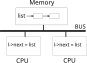
\includegraphics[scale=0.8]{fig/smp.pdf}
\caption{Simplified SMP architecture}
\label{fig:smp}
\end{figure}

As an example of why we need locks, consider two processes
with exited children calling
the {\tt wait} system call on two different
CPUs.  {\tt wait} frees the child's memory.
Thus
on each CPU, the kernel will free physical pages.
The page allocator maintains a linked
list of free pages:
allocating a page pops from the head of the free list
(see \texttt{kernel/page\_allocator.h}, \texttt{page\_allocator::alloc}),
and freeing a page pushes a page onto the list
(see \texttt{kernel/page\_allocator.h}, \texttt{page\_allocator::free}).
For best performance, we might hope that the frees of the two parent processes
would execute in parallel without either having to wait for the other,
but this would not be correct given a naive free-list implementation.

Figure~\ref{fig:smp} illustrates the setting in more detail: the
linked list of free pages is in memory that is shared by the two CPUs, which
manipulate the list using load and store instructions. (In
reality, the processors have caches, but conceptually
multiprocessor systems behave as if there were a single, shared memory.)
If there were no concurrent
requests, you might implement a list \lstinline{push} operation as
follows:
\begin{lstlisting}[numbers=left,firstnumber=1]
    struct element {
      int data;
      struct element *next;
    };

    struct element *list = 0;

    void
    push(int data)
    {
      struct element *l;

      l = malloc(sizeof *l);
      l->data = data;
      l->next = list; (*@\label{line:next}@*)
      list = l;  (*@\label{line:list}@*)
    }
\end{lstlisting}

\begin{figure}[t]
\center
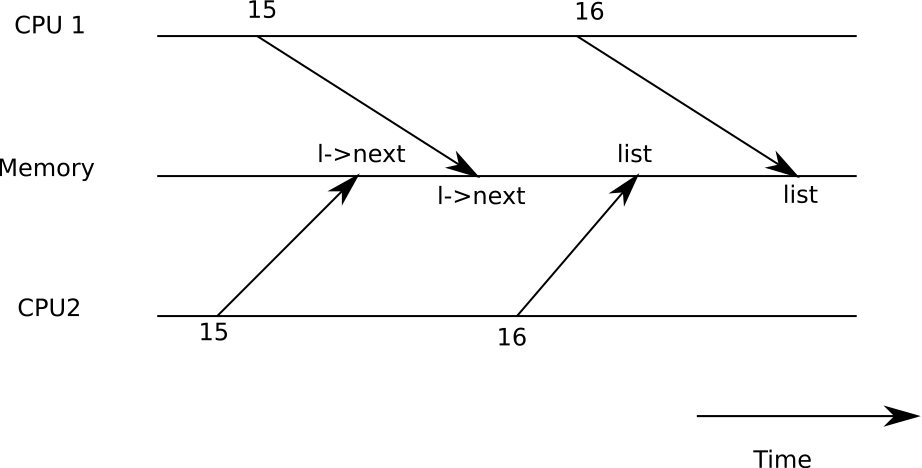
\includegraphics[scale=0.5]{fig/race.pdf}
\caption{Example race}
\label{fig:race}
\end{figure}

This implementation is correct if executed in isolation.
However, the code is not correct if more than one
copy executes concurrently.
If two CPUs execute
\lstinline{push}
at the same time,
both might execute line~\ref{line:next} as shown in Fig~\ref{fig:smp},
before either executes line~\ref{line:list}, which results
in an incorrect outcome as illustrated by Figure~\ref{fig:race}.
There would then be two
list elements with
\lstinline{next}
set to the same former value of
\lstinline{list}.
When the two assignments to
\lstinline{list}
happen at line~\ref{line:list},
the second one will overwrite the first;
the element involved in the first assignment
will be lost.

The lost update at line~\ref{line:list} is an example of a
\indextext{race}.
A race is a situation in which a memory location is accessed
concurrently, and at least one access is a write.
A race is often a sign of a bug, either a lost update
(if the accesses are writes) or a read of
an incompletely-updated data structure.
The outcome of a race depends on
the machine code generated by the compiler,
the timing of the two CPUs involved,
and how their memory operations are ordered by the memory system,
which can make race-induced errors difficult to reproduce
and debug.
For example, adding print statements while debugging
\lstinline{push}
might change the timing of the execution enough
to make the race disappear.

The usual way to avoid races is to use a lock.
Locks ensure
\indextext{mutual exclusion},
so that only one CPU at a time can execute
the sensitive lines of
\lstinline{push};
this makes the scenario above impossible.
The sequence of instructions in between acquiring and releasing a lock
is often called a
\indextext{critical section}.
When a lock is associated with a shared structure, we say the lock
protects that structure.

When we say that a lock protects data, we really mean
that the lock protects some collection of invariants
that apply to the data.
Invariants are properties of data structures that
are maintained across operations.
Typically, an operation's correct behavior depends
on the invariants being true when the operation
begins. The operation may temporarily violate
the invariants but must reestablish them before
finishing.
For example, in the linked list case, the invariant is that
\lstinline{list}
points at the first element in the list
and that each element's
\lstinline{next}
field points at the next element.
The implementation of
\lstinline{push}
violates this invariant temporarily: in line~\ref{line:next},
\lstinline{l}
points
to the next list element, but
\lstinline{list}
does not point at
\lstinline{l}
yet (reestablished at line~\ref{line:list}).
The race we examined above
happened because a second CPU executed
code that depended on the list invariants
while they were (temporarily) violated.
Proper use of a lock ensures that only one CPU at a time
can operate on the data structure in the critical section, so that
no CPU will execute a data structure operation when the
data structure's invariants do not hold.

You can think of a lock as
\indextext{serializing}
concurrent critical sections so that they run one at a time,
and thus preserve invariants (assuming the critical sections
are correct in isolation).
You can also think of critical sections guarded by the same lock as being
atomic with respect to each other,
so that each sees only the complete set of
changes from earlier critical sections, and never sees
partially-completed updates.

Though useful for correctness, locks inherently
limit performance. For example, if two processes free pages
concurrently, locks may serialize the two critical sections,
so that there is no
benefit from running them on different CPUs. We say that multiple
processes \indextext{conflict} if they want the same lock at the same
time, or that the lock experiences \indextext{contention}. A major
challenge in kernel design is avoidance of lock contention
in pursuit of parallelism. xv6++ does
little of that, but sophisticated kernels organize
data structures and algorithms specifically to avoid lock contention.
For example, a kernel may maintain a separate free list per CPU and only touch
another CPU's free list if the current CPU's list is empty and it must steal
memory from another CPU. Other use cases may require more
complicated designs.

%% 
\section{Code: Locks}
%% 

Please read (see \texttt{kernel/spin\_lock.h}, \texttt{class spin\_lock})
and (see \texttt{kernel/sleep\_lock.h}, \texttt{class sleep\_lock}).

xv6++ has two types of locks: spin locks and sleep locks.
We'll start with spin locks.
A spin lock provides mutual exclusion by busy-waiting (spinning)
until the lock becomes available.
In xv6++, locks share a small common base that tracks whether the lock is held
(see \texttt{kernel/lock\_base.h}, \texttt{class lock\_base}).

A naive attempt to acquire a lock might look like it tests whether the lock
is free and then marks it held. Unfortunately, such a two-step approach does not
guarantee mutual exclusion on a multiprocessor: two CPUs could simultaneously
observe that the lock is free and both decide they acquired it.
What we need is a way to combine ``test'' and ``set'' into a single
\indextext{atomic}
(i.e., indivisible) step.

Because locks are widely used,
multi-core processors usually provide an instruction that
can be used to make the test-and-set atomic.
On RISC-V, this can be done with atomic memory operations.
C and C++ provide built-ins that compile to the needed atomic instructions.
xv6++'s spin lock acquire path uses atomic operations to set the lock word
and determine whether it was previously free
(see \texttt{kernel/spin\_lock.h}, \texttt{spin\_lock::acquire}).

Once the lock is acquired, xv6++ records (for debugging) which CPU holds the lock
(see \texttt{kernel/spin\_lock.h}, \texttt{spin\_lock::holding}).

Releasing a spin lock clears the owner and makes the lock available again
(see \texttt{kernel/spin\_lock.h}, \texttt{spin\_lock::release}).

%% 
\section{Code: Using locks}
%% 

xv6++ uses locks in many places to avoid races.
The page allocator is a good example: allocating and freeing pages
manipulates shared state (the free list), so it is protected by a lock
(see \texttt{kernel/page\_allocator.h}, \texttt{page\_allocator::alloc})
and (see \texttt{kernel/page\_allocator.h}, \texttt{page\_allocator::free}).
If those operations omitted locking, concurrent alloc/free calls could corrupt
the free list.

A hard part about using locks is deciding how many locks
to use and which data and invariants each lock should protect.
There are a few basic principles.
First, any time a variable can be written by one CPU
at the same time that another CPU can read or write it,
a lock should be used to keep the two
operations from overlapping.
Second, remember that locks protect invariants:
if an invariant involves multiple memory locations,
typically all of them need to be protected
by a single lock to ensure the invariant is maintained.

The rules above say when locks are necessary but say nothing about when locks
are unnecessary, and it is important for efficiency not to lock too much,
because locks reduce parallelism. If parallelism isn't important, then one
could arrange to have only a single thread and not worry about locks.
A simple kernel can do this on a multiprocessor by having a single lock;
the kernel acquires the lock every time the kernel is entered
from user space, for a system call or interrupt;
the kernel releases the lock when it returns to user space.
This ``big kernel lock'' approach sacrifices parallelism: only one
CPU can execute in the kernel at a time.

As an example of coarse-grained locking, xv6++'s page allocator has a single free list
protected by a single lock. If multiple processes on different CPUs try to allocate pages
at the same time, each may have to wait in the lock acquire path.
If contention for the lock wasted a significant fraction of CPU time,
performance could be improved by changing the allocator to have a separate free list
per CPU, each with its own lock, to allow truly parallel allocation.

As an example of fine-grained locking, xv6++ has separate locks for many distinct objects,
so that unrelated operations can often proceed without waiting.
For example, each process has its own lock protecting its state
(see \texttt{kernel/process.h}, \texttt{class process}),
each cached disk buffer has its own sleep lock
(see \texttt{kernel/buffer\_cache.h}, \texttt{struct buf}),
and each in-memory inode has its own sleep lock
(see \texttt{kernel/file\_system.h}, \texttt{struct inode}).

As subsequent chapters explain each part of xv6++, they
will mention examples of xv6++'s use of locks
to deal with concurrency.
As a preview,
Figure~\ref{fig:locktable}
lists many of the locks in xv6++.

\begin{figure}[t]
\center
\begin{tabular}{ll}
{\bf Lock} & {\bf Description} \\
\midrule
\texttt{kernel.cache.lock} & Protects allocation and LRU management of block buffer cache entries \\
\texttt{kernel.console.lock} & Serializes console input state updates and readers \\
\texttt{kernel.console\_driver.lock} & Serializes access to UART transmit/receive state \\
\texttt{kernel.fmanager.file\_lock} & Serializes allocation of a \texttt{file} in the global file table \\
\texttt{kernel.fmanager.pipe\_lock} & Serializes allocation and updates of pipes \\
\texttt{kernel.fsystem.inode\_lock} & Protects allocation of in-memory inode entries \\
\texttt{kernel.disk\_driver.vdisk\_lock} & Serializes access to disk hardware and the virtio descriptor state \\
\texttt{kernel.allocator.lock} & Serializes allocation of physical memory pages \\
\texttt{kernel.log.lock} & Serializes operations on the transaction log \\
\texttt{kernel.processes.pid\_lock} & Serializes increments of \texttt{next\_pid} \\
\texttt{kernel.processes.wait\_lock} & Helps \texttt{wait} avoid lost wakeups \\
\texttt{kernel.processes.lock} & Protects the global process table \\
\texttt{process.lock} & Serializes changes to a process's state \\
\texttt{kernel.interrupts.ticks\_lock} & Serializes operations on the ticks counter \\
\texttt{inode.lock} & Serializes operations on each inode and its content \\
\texttt{buf.lock} & Serializes operations on each cached disk buffer \\
\end{tabular}
\caption{Locks in xv6++}
\label{fig:locktable}
\end{figure}

%% 
\newpage
\section{Deadlock and lock ordering}
%% 

Suppose the functions running on CPUs C1 and C2 both have a point at
which each needs to hold both lock A and lock B, and they acquire them
in different orders:

\begin{center}
  \input{fig/order.tex}
\end{center}

With a bit of bad luck, C1 and C2 might both execute their first
acquire at exactly the same moment; both can succeed, since they are
asking for different locks. But then both C1 and C2 will have to wait
in their second calls to acquire, since both locks are already
held by the other CPU. Because both CPUs are waiting for each
other, neither will ever release a lock, and both will wait forever.
This situation is called \indextext{deadlock}.

The key problem in the C1/C2 example is that the two CPUs acquired
the locks in different orders. If they had both tried to acquire A
first, one would have acquired A and then B and then released them both,
and then the other CPU could have proceeded. More generally,
locking code must follow this rule to avoid deadlock: all code paths
that hold multiple locks must acquire locks in the same order. The
need for this global lock acquisition order means that locks are
effectively part of each function's specification: callers must invoke
functions in a way that causes locks to be acquired in the agreed-on
order.

Honoring a global deadlock-avoiding order can be surprisingly
difficult. Sometimes the lock order conflicts with logical program
structure. Sometimes the identities of locks aren't known in advance,
perhaps because one lock must be held in order to discover the identity
of the lock to be acquired next. This kind of situation arises in the
file system as it looks up successive components in a path name, and
in the code for the {\tt wait} and {\tt exit} system calls
as they search the table of
processes looking for child processes. Finally, the danger of deadlock
is often a constraint on how fine-grained one can make a locking
scheme, since more locks often means more opportunity for deadlock.
The need to avoid deadlock is often a major factor in kernel
implementation.

A question that sometimes arises is what should happen if a CPU tries
to acquire a lock that the same CPU already holds. One line of
reasoning is that this should be allowed: no other CPU can hold the
lock, so there's no need to worry about CPUs interfering with each
others' use of the protected data. Locking systems that allow a CPU to
re-acquire a lock it already holds are called {\it re-entrant} or {\it
recursive}. On the other hand, if a lock is already held, even on
the same CPU, that means an operation may have temporarily violated
and not yet restored some invariants; to allow a new operation to
commence while the invariants don't hold seems like an invitation to
bugs. xv6++ takes this latter view, and forbids a CPU that currently
holds a lock from re-acquiring it. Detecting this situation is one purpose
of the lock ``holding'' checks in the spin lock implementation
(see \texttt{kernel/spin\_lock.h}, \texttt{spin\_lock::holding}).

\section{Locks and interrupts}
\label{s:lockinter}

Some xv6++ spin locks protect data that is used by
both threads and interrupt handlers.
For example, the timer interrupt path increments the system tick counter
(see \texttt{kernel/interrupt\_manager.h}, \texttt{clock\_tick})
at about the same time that a kernel
thread reads the tick counter in a sleep call
(see \texttt{kernel/interrupt\_manager.h}, \texttt{sleep}).
The lock protecting the tick counter serializes those accesses
(see \texttt{kernel/interrupt\_manager.h}, \texttt{ticks\_lock}).

The interaction of spin locks and interrupts raises a potential danger.
Suppose a kernel thread holds a spin lock, and its CPU is interrupted.
If the interrupt handler tries to acquire the same spin lock, it will spin
waiting for it to be released. But the lock will never be released,
because the interrupted code cannot continue until the interrupt handler returns.
The CPU will deadlock.

To avoid this situation, if a spin lock is used by an interrupt handler,
a CPU must never hold that lock with interrupts enabled.
xv6++ follows the common approach of disabling interrupts while holding
spin locks, and restoring the prior interrupt state when the CPU is no longer
holding any spin locks. The per-CPU interrupt disable/restore nesting is managed
by the CPU manager
(see \texttt{kernel/cpu\_manager.h}, \texttt{push\_off})
and (see \texttt{kernel/cpu\_manager.h}, \texttt{pop\_off}).
The low-level enable/disable primitives ultimately manipulate RISC-V
control registers
(see \texttt{kernel/riscv.h}, \texttt{intr\_off})
and (see \texttt{kernel/riscv.h}, \texttt{intr\_on}).

It is important that interrupt disabling occurs before a spin lock is made
visible as held, and that interrupt restoration occurs only after releasing
the lock; otherwise there can be a brief window when a lock is held with
interrupts enabled, and an unfortunately timed interrupt can deadlock the system.

%% 
\section{Instruction and memory ordering}
%% 

It is natural to think of programs executing in the order
in which source code statements appear.
That's a reasonable mental model for single-threaded
code, but is incorrect when
multiple threads interact through shared memory~\cite{riscv:user,boehm04}.
One reason is that compilers emit load and store
instructions in orders different from those implied
by the source code, and may entirely omit them
(for example by caching data in registers).
Another reason is that the CPU may execute instructions
out of order to increase performance.

As an example of what could go wrong,
it would be a disaster if the compiler or CPU moved a store that publishes
a pointer to a newly-initialized object to a point before the object is
fully initialized, or moved a store that updates a shared structure to a
point after the lock release.
In that case, another CPU could acquire the lock and observe a partially
initialized or partially updated structure.

The good news is that compilers and CPUs help concurrent programmers
by following a set of rules called the \indextext{memory model}, and
by providing primitives to help programmers control re-ordering.
Lock implementations typically include appropriate ordering constraints
so that memory operations in a critical section are not reordered across
lock acquire or release.

%% 
\section{Sleep locks}
%% 

Sometimes xv6++ needs to hold a lock for a long time. For example, the
file system keeps an inode locked while reading and writing its content
on the disk, and these disk operations can take tens of milliseconds.
Holding a spin lock that long would lead to waste if another process wanted to
acquire it, since the acquiring process would waste CPU for a long time while
spinning. Another drawback of spin locks is that a process cannot yield the CPU
while retaining a spin lock.

xv6++ provides locks that are suitable for long operations in the form of
\indextext{sleep locks}
(see \texttt{kernel/sleep\_lock.h}, \texttt{class sleep\_lock}).
A sleep lock uses an internal spin lock to protect its state, and when a thread
must wait it sleeps (yielding the CPU) until the lock becomes available.
Because sleep locks allow sleeping, they leave interrupts enabled while held, and
thus cannot be used in interrupt handlers. Also, because acquiring a sleep lock
may sleep, sleep locks cannot be acquired while holding a spin lock.

Spin locks are best suited to short critical sections,
since waiting for them wastes CPU time;
sleep locks work well for lengthy operations.

%% 
\section{Real world}
%% 

Programming with locks remains challenging despite years of research
into concurrency primitives and parallelism.
It is often best to conceal locks within
higher-level constructs like synchronized queues, although xv6++ does not
do much of this. If you program with locks, it is wise to use a tool that attempts to
identify races, because it is easy to miss an invariant that requires
a lock.

It is possible to implement locks without atomic
instructions~\cite{lamport:bakery}, but it is expensive, so most
operating systems use atomic instructions.

Locks can be expensive if many CPUs try to acquire the same lock
at the same time. If one CPU has a lock cached in its local cache, and another CPU
must acquire the lock, then the atomic instruction to update the cache line that
holds the lock must move the line from the one CPU's cache to the other CPU's cache,
and perhaps invalidate any other copies of the cache line. Fetching a cache line from
another CPU's cache can be orders of magnitude more expensive than
fetching a line from a local cache.

To avoid the expenses associated with locks, many operating systems
use lock-free data structures and algorithms~\cite{herlihy:art,mckenney:rcuusage}.
Lock-free programming is more complicated than programming with locks, however,
since one must worry about instruction and memory reordering and safe memory
reclamation. xv6++ avoids the additional complexity of lock-free programming.

%% 
\section{Exercises}
%% 

\begin{enumerate}

\item Comment out the locking in the page allocator's allocation path
(see \texttt{kernel/page\_allocator.h}, \texttt{page\_allocator::alloc}).
This seems like it should cause problems for
kernel code that allocates pages;
what symptoms do you expect to see?
When you run xv6++, do you see these symptoms?
If you don't see a problem, why not?
See if you can provoke a problem by inserting
dummy loops into the critical section of the allocator.

\item Suppose that you instead commented out the
locking in the page allocator's free path
(see \texttt{kernel/page\_allocator.h}, \texttt{page\_allocator::free}).
What might now go wrong? Is lack of locks in freeing
less harmful than in allocating?

\item If two CPUs allocate pages
at the same time, one may have to wait for the other,
which is bad for performance.
Modify the allocator
to have more parallelism, so that simultaneous
allocations from different CPUs can proceed without waiting for each other.

\item Write a parallel program using POSIX threads, which is supported on most
operating systems. For example, implement a parallel hash table and measure if
the number of puts/gets scales with increasing number of CPUs.

\end{enumerate}

% LocalWords:  CPUs uniprocessor interruptible allocator invariants spinlock
% LocalWords:  amoswap SMP deadlock ordering cacheline PLIC DMA POSIX Pthreads
